\newpage
\section{Sensitivity Analysis and Error Analysis}%有时间再做（没时间删去，影响不大）

\subsection{Sensitivity Analysis}
%灵敏度分析用于评估模型输入参数变化对输出结果的影响程度，识别关键参数

本研究的核心结论依赖于两个层次的敏感性：其一是Q1中观众偏好强度的后验推断是否稳定；其二是Q2--Q4中不同淘汰机制在多目标指标下的相对优势是否会在压力测试下发生结构性反转。为此，我们采用“可视化诊断 + 反事实对比 + 压力测试曲线”三种方式进行灵敏度分析。

\paragraph{Q1后验不确定性与可识别性}
我们首先通过不确定性热力图展示每个赛季-周在Percent机制下的推断区间宽度，观察哪些周对参数与噪声更敏感（图\ref{fig:q1_uncertainty_heatmap}）。随后，结合Q1结果区间图（见图\ref{fig:q1_fan_share_intervals}）检验“高评委分但低观众支持”的典型结构是否被模型捕捉。

为保证论文表格可复现，本文中以\texttt{paper\_*.csv}形式插入的“裁剪版表格”均由主线输出确定性导出（导出脚本：\texttt{src/mcm2026/pipelines/mcm2026c\_export\_paper\_tables.py}），其上游来源分别为\texttt{outputs/tables/mcm2026c\_q1\_uncertainty\_summary.csv}、\texttt{outputs/tables/mcm2026c\_q1\_error\_diagnostics\_week.csv}、\texttt{outputs/tables/mcm2026c\_q2\_mechanism\_comparison.csv}与\texttt{outputs/tables/mcm2026c\_q4\_sensitivity\_summary.csv}。

\begin{table}[H]
    \centering
    \caption{Q1高不确定性周：以有效样本量占比（ESS ratio）与证据强度（evidence）筛选最不稳定的周段，用于定位误差高风险输入。}
    \label{tab:q1_high_uncertainty_weeks}
    \pgfplotstabletypeset[
        col sep=comma,
        columns={season,week,nactive,nexit,essratio,evidence},
        columns/season/.style={column name=Season},
        columns/week/.style={column name=Week},
        columns/nactive/.style={column name={$n_{active}$}},
        columns/nexit/.style={column name={$n_{exit}$}},
        columns/essratio/.style={column name=ESS ratio, fixed, precision=3},
        columns/evidence/.style={column name=Evidence, fixed, precision=3},
        every head row/.style={before row=\toprule, after row=\midrule},
        every last row/.style={after row=\bottomrule},
    ]{../outputs/tables/paper_q1_high_uncertainty_weeks.csv}
\end{table}

\begin{figure}[H]
    \centering
    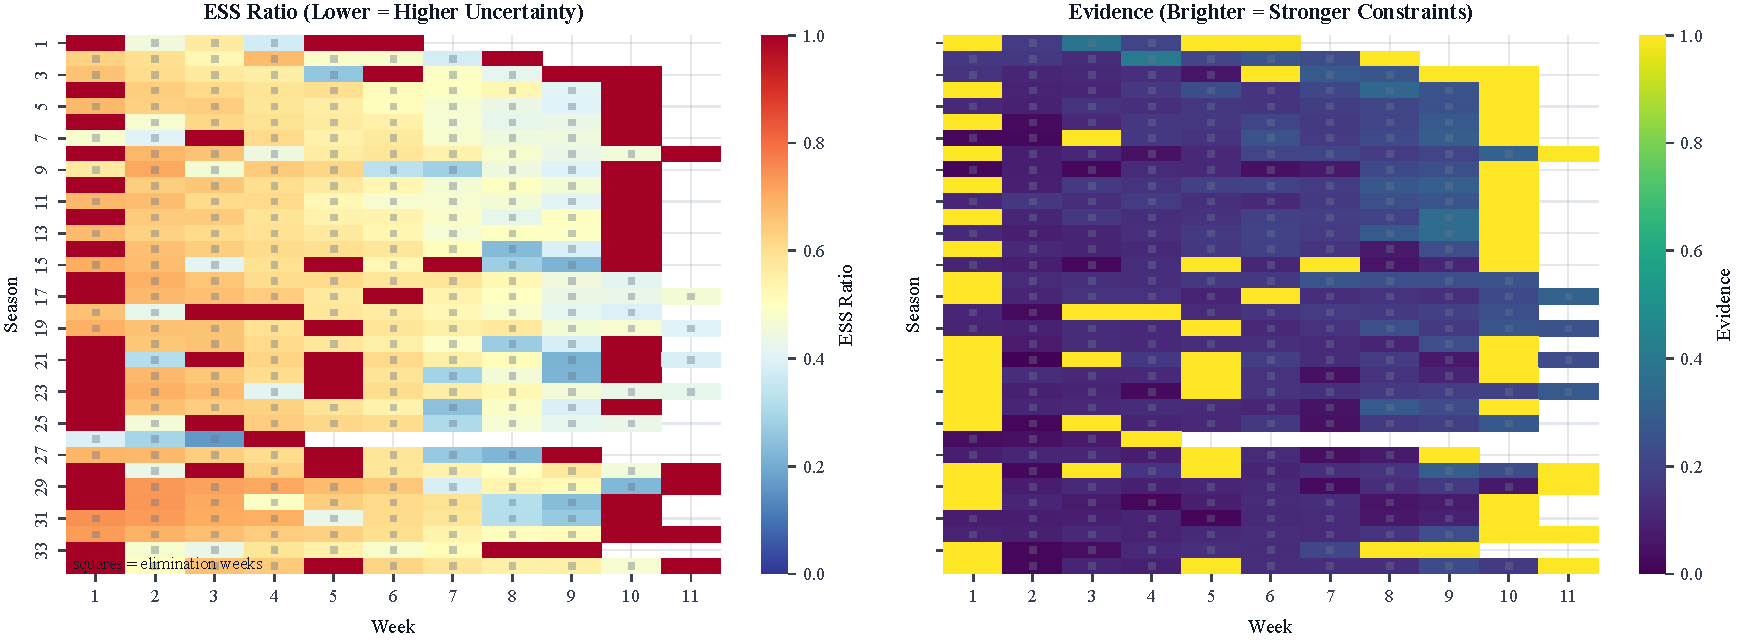
\includegraphics[width=0.92\linewidth]{../outputs/figures/q1/pdf/q1_uncertainty_heatmap.pdf}
    \caption{Q1不确定性诊断：Percent机制下的赛季-周不确定性热力图。}
    \label{fig:q1_uncertainty_heatmap}
\end{figure}

\begin{table}[H]
    \centering
    \caption{Q2机制分歧摘要：按Percent与Rank差异周数（diff weeks）排序，汇总每个赛季的机制匹配率，用于选择最能区分机制的“高价值验证赛季”。}
    \label{tab:q2_divergence_summary}
    \pgfplotstabletypeset[
        col sep=comma,
        columns={season,nweeks,diffweeks,matchpercent,matchrank,matchpercentjs},
        columns/season/.style={column name=Season},
        columns/nweeks/.style={column name=$n_{weeks}$},
        columns/diffweeks/.style={column name=Diff weeks},
        columns/matchpercent/.style={column name=Match(Percent), fixed, precision=3},
        columns/matchrank/.style={column name=Match(Rank), fixed, precision=3},
        columns/matchpercentjs/.style={column name=Match(Percent+JS), fixed, precision=3},
        every head row/.style={before row=\toprule, after row=\midrule},
        every last row/.style={after row=\bottomrule},
    ]{../outputs/tables/paper_q2_divergence_summary.csv}
\end{table}

\paragraph{机制差异对关键周的敏感性}
不同投票汇总机制（Percent与Rank）可能在特定“分歧周”产生显著不同的淘汰结果。我们通过机制敏感性总览图对这种差异进行聚合展示，刻画差异大小在赛季-周维度的分布（图\ref{fig:q1_mechanism_sensitivity_overview}）。进一步地，使用周层分歧热力图定位差异最集中的周段，为Q2的反事实模拟提供“高价值验证点”（图\ref{fig:q2_week_level_divergence_heatmap}）。

\begin{figure}[H]
    \centering
    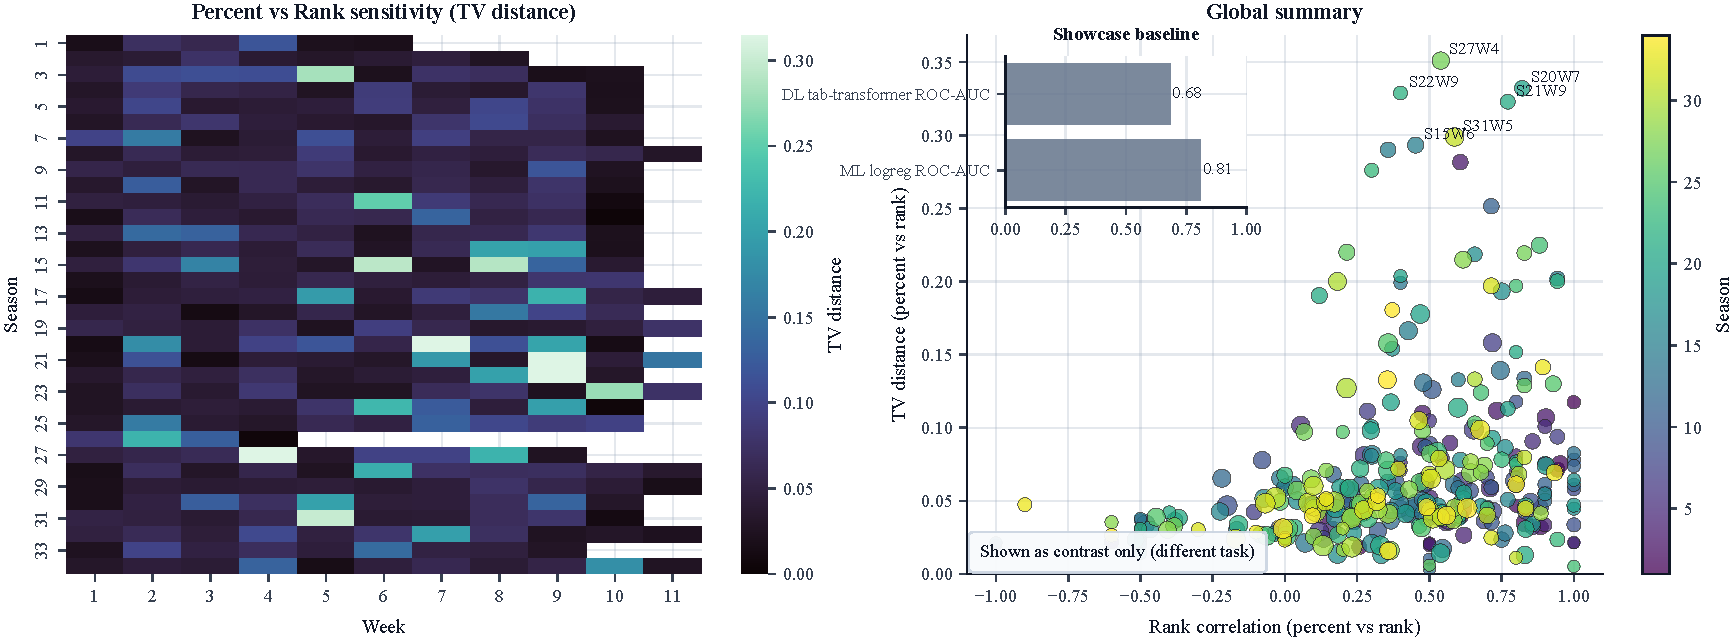
\includegraphics[width=0.96\linewidth]{../outputs/figures/q1/pdf/q1_mechanism_sensitivity_overview.pdf}
    \caption{机制敏感性总览：在赛季-周尺度衡量Percent与Rank引入的结构性差异。}
    \label{fig:q1_mechanism_sensitivity_overview}
\end{figure}

\begin{figure}[H]
    \centering
    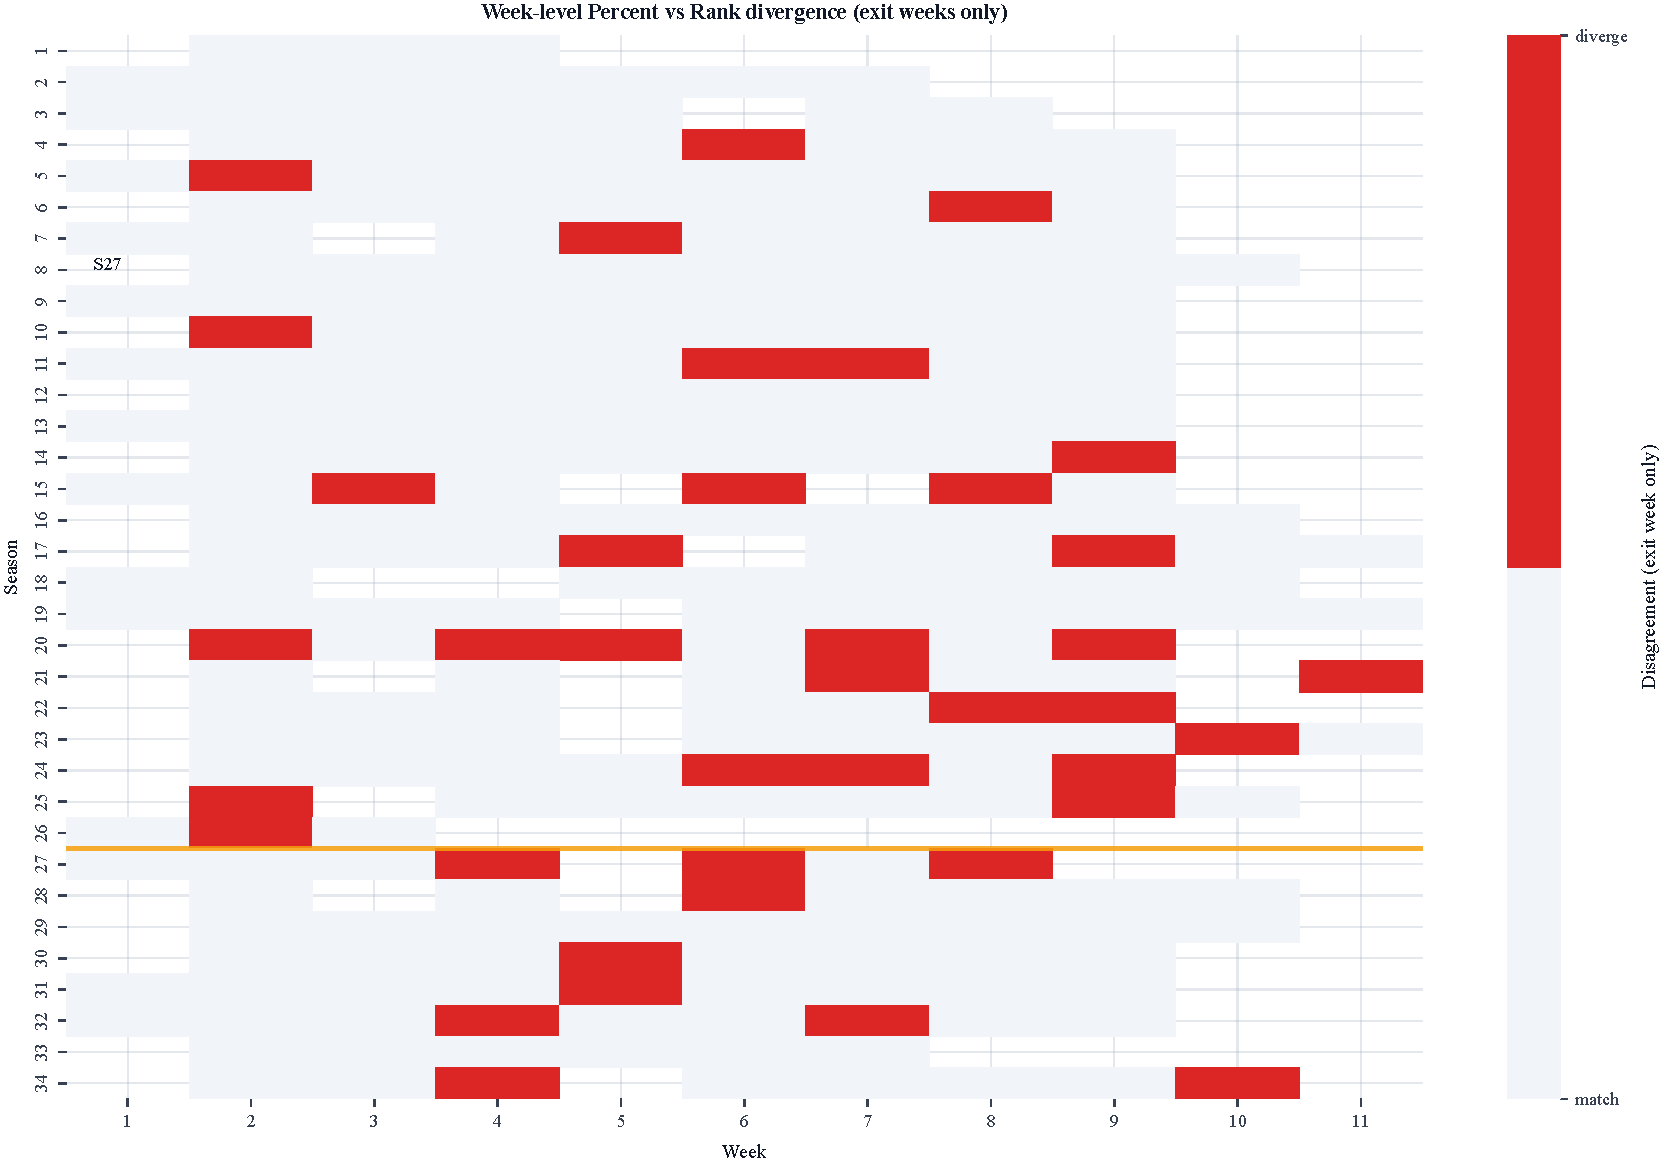
\includegraphics[width=0.96\linewidth]{../outputs/figures/q2/pdf/q2_week_level_divergence_heatmap.pdf}
    \caption{周层分歧定位：识别Percent与Rank机制在何时产生最大分歧，为反事实分析提供切入点。}
    \label{fig:q2_week_level_divergence_heatmap}
\end{figure}

在周层定位之外，我们也从整体分布角度检验“机制差异是否集中在少数极端周”，以避免仅凭个例得出结论。图\ref{fig:q2_mechanism_difference_distribution}给出了关键差异指标的分布形态，便于判断差异是系统性的还是偶发性的。

\begin{figure}[H]
    \centering
    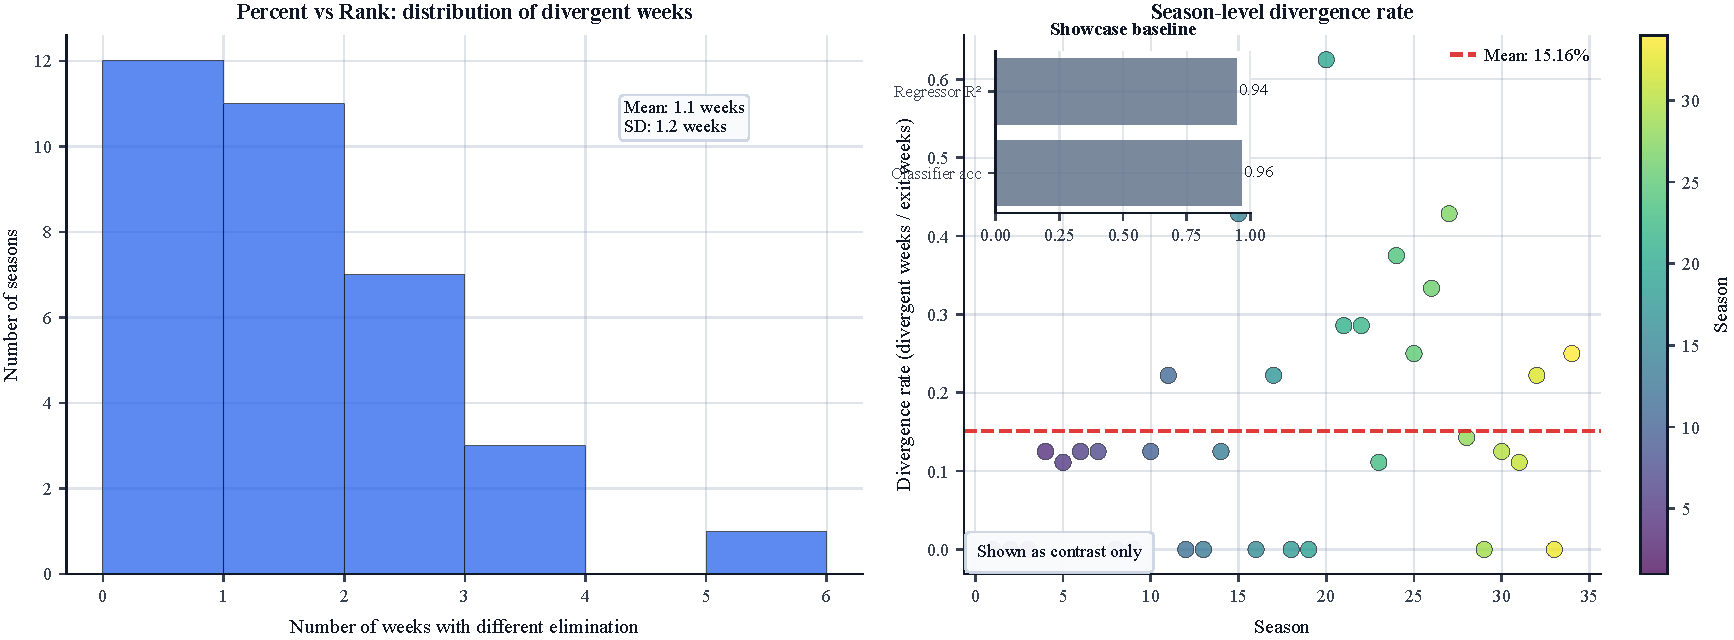
\includegraphics[width=0.92\linewidth]{../outputs/figures/q2/pdf/q2_mechanism_difference_distribution.pdf}
    \caption{机制差异分布：对比Percent与Rank在关键差异指标上的整体分布形态。}
    \label{fig:q2_mechanism_difference_distribution}
\end{figure}


\subsection{Error Analysis for Question 1}
%最终数值结果的正确性或合理性是第一位的；对数值结果或模拟结果进行必要的检验。结果不正确、不合理、或误差大时，分析原因，对算法、计算方法、或模型进行修正、改进；

针对Q1，我们主要从三方面控制误差：
\begin{enumerate}[label=(\arabic*),leftmargin=2.4em]
    \item \textbf{数值稳定性：}对后验重采样次数进行充分设置，确保区间估计收敛；并在每个赛季-周检查有效样本量与区间宽度，避免由极端权重导致的数值不稳。
    \item \textbf{方向性合理性：}通过“评委信号与观众信号的相关性”检查模型不会系统性地产生反直觉输出（例如所有周都推断评委与观众高度一致）。
    \item \textbf{一致性核验：}对关键周（淘汰与高分歧周）进行人工核查，确认输入字段与淘汰标记无偏差。
\end{enumerate}

\begin{table}[H]
    \centering
    \caption{Q1误差诊断样例：对存在淘汰的周，列出观众-评委排序相关性与“观察到的淘汰选手在后验均值下的退出概率”，用于发现模型在低可识别周的偏差模式。}
    \label{tab:q1_error_cases}
    {\small
    \pgfplotstabletypeset[
        col sep=comma,
        columns={season,week,nactive,corr,observedexit,pexit},
        columns/season/.style={column name=Season},
        columns/week/.style={column name=Week},
        columns/nactive/.style={column name={$n_{active}$}},
        columns/corr/.style={column name={Corr(judge,fan)}, fixed, precision=2},
        columns/observedexit/.style={column name=Observed exit, string type, column type=p{5.6cm}},
        columns/pexit/.style={column name={$P(\mathrm{exit}|\mathrm{posterior\ mean})$}, fixed, precision=3},
        every head row/.style={before row=\toprule, after row=\midrule},
        every last row/.style={after row=\bottomrule},
    ]{../outputs/tables/paper_q1_error_cases.csv}
    }
\end{table}





\subsection{Error Analysis for Question 2}

针对Q2的反事实模拟，我们将误差分解为“机制差异”与“随机性差异”。前者通过固定同一赛季周度数据进行机制替换来控制；后者通过多次重复模拟并报告跨模拟的方差来度量。与此同时，Q4中引入的压力测试曲线可视为对Q2结果的外推检验：若在异常冲击增强后某机制的表现仍保持相对优势，则说明结论对数据扰动更稳健（图\ref{fig:q4_robustness_curves}）。

此外，我们单独评估了“Judge Save”这一规则变体对结果稳定性的影响，作为对Q2误差来源（规则细节变化）的一次对照试验（图\ref{fig:q2_judge_save_impact}）。

\begin{figure}[H]
    \centering
    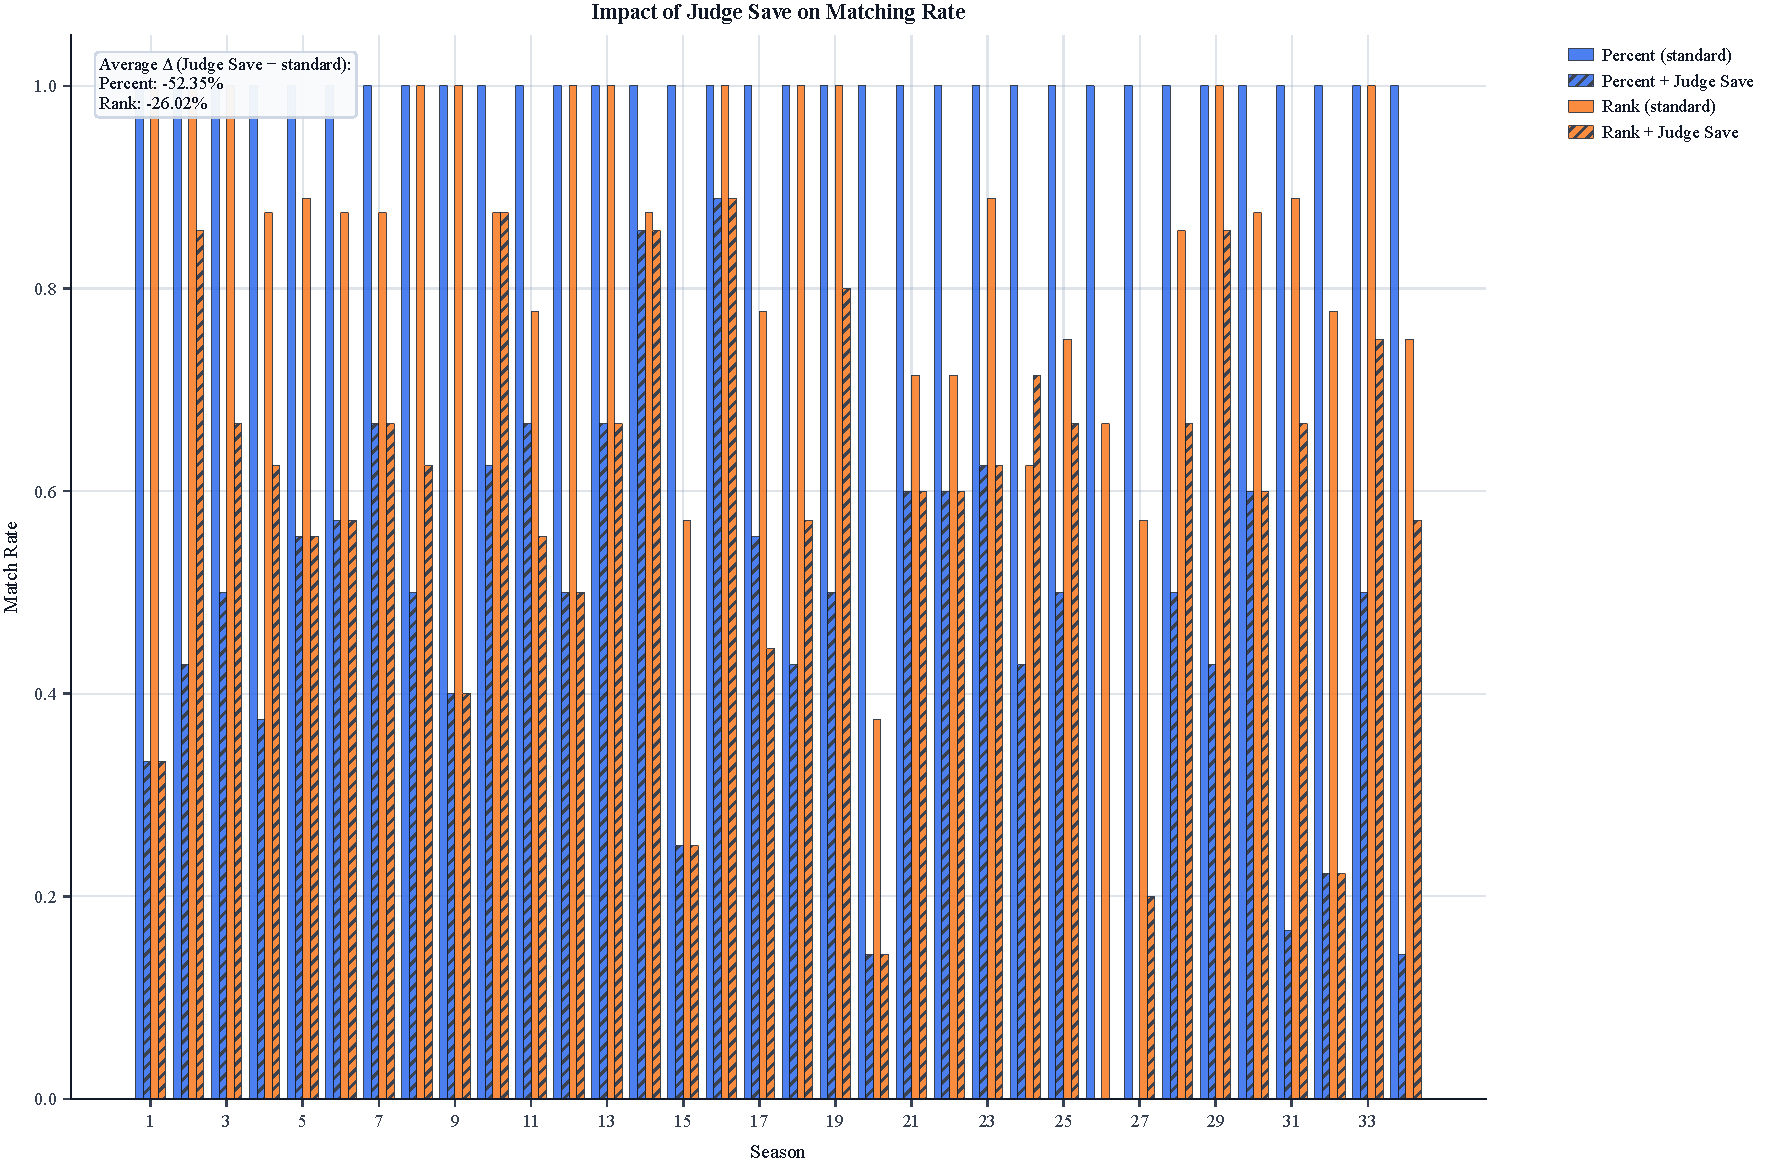
\includegraphics[width=0.92\linewidth]{../outputs/figures/q2/pdf/q2_judge_save_impact.pdf}
    \caption{规则变体对照：Judge Save机制对关键结果的影响，用于评估规则细节变化带来的误差敏感性。}
    \label{fig:q2_judge_save_impact}
\end{figure}

\begin{figure}[H]
    \centering
    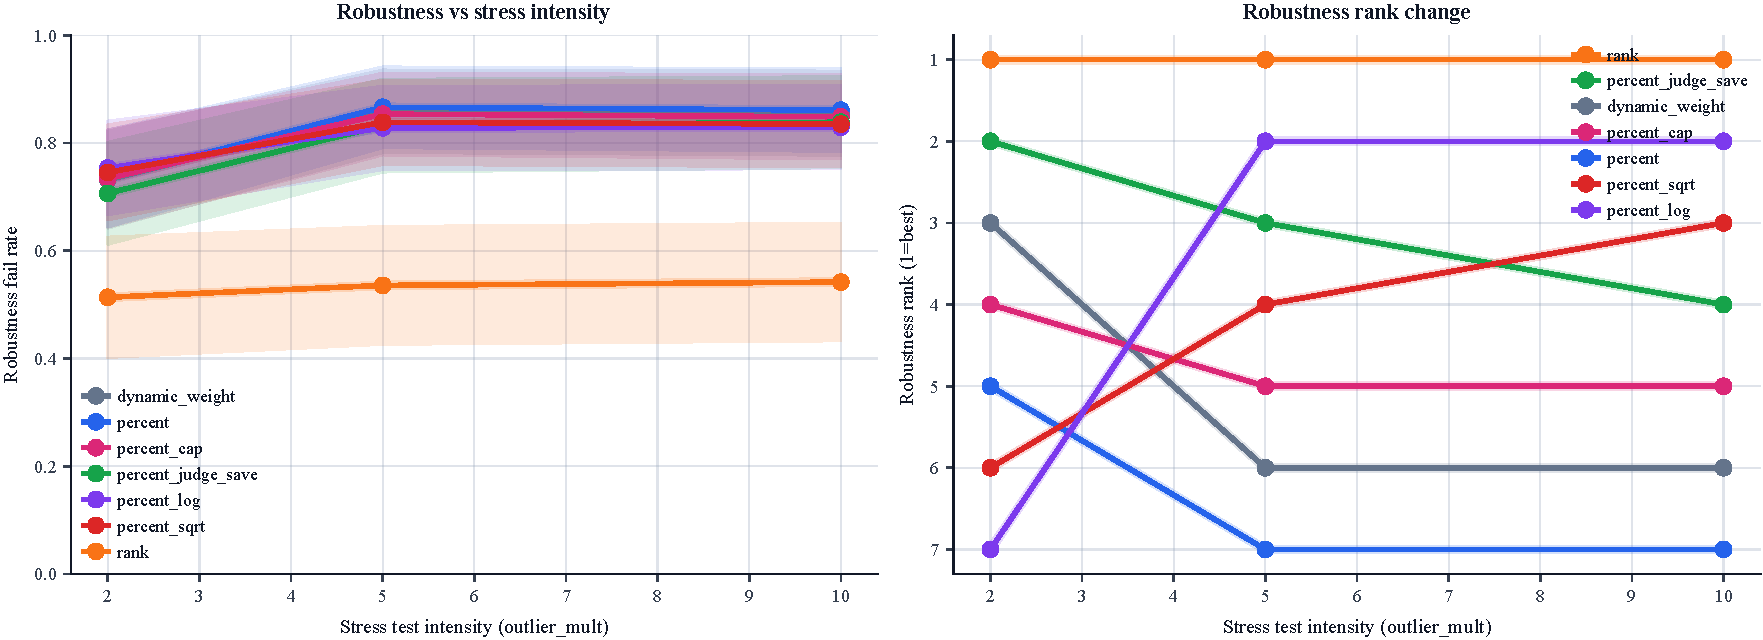
\includegraphics[width=0.96\linewidth]{../outputs/figures/q4/pdf/q4_robustness_curves.pdf}
    \caption{压力测试与误差外推：不同机制在异常冲击强度变化下的鲁棒性失败率与排名变化。}
    \label{fig:q4_robustness_curves}
\end{figure}
